\chapter{Аналитический раздел}
В этом разделе будет приведено описание модели трёхмерного объекта в сцене,
рассмотрены формализация объектов сцены и требования к работе программы.
Будут рассмотрены алгоритмы построения трёхмерного изображения, методы закраски, модели освещения, а также способы текстуризации и закраски треугольников.

\section{Описание модели трёхмерного объекта в сцене}
Модель трёхмерного объекта в сцене в работе представлена в виде полигональной сетки.

Полигональная сетка -- совокупность вершин, рёбер и граней, которые определяют форму многогранного объекта в трёхмерной компьютерной графике.
Сетка может состоять из граней произвольной формы, но в курсовой работе грани имеют форму треугольников, так как любой полигон 
произвольной можно представить как треугольник.

Такой способ является универсальным, так как позволяет описывать трёхмерные объекты произвольной формы.
Количество полигонов напрямую влияет на реалистичность визуализации модели, но при этом обработка большого количества граней
приводит к увеличению требований к системным ресурсам.

Так как полигоны задают плоскости, то для достижения эффекта неровности можно изменять нормали к поверхностям.
При создании модели также нужно указать текстурные координаты.

\section{Формализация объектов синтезируемой сцены}
Сцена состоит из следующих объектов:
\begin{enumerate}
	\item Геометрический объект -- представляется в виде полигональной сетки. 
	В число рассматриваемых геометрических объектов входит куб, сфера, цилиндр и конус.
	Для описания геометрического объекта требуется указать координаты вершин, ребра и грани между ними,
	цвет объекта или текстура, которая его покрывает, а также свойства поверхности: коэффициент отражения,
	коэффициент прозрачности и коэффициент блеска.
	\item Источник света -- представляется в виде вектора направления света. 
	Также у источника света есть следующие характеристики: место расположения, цвет и интенсивность излучения. 
	\item Камера - характеризуется своим пространственным положением и направлением просмотра.
\end{enumerate}

Остальное пространство также представлено интенсивностью окружающего света и его цветом.

\section{Требования к работе программы}
Программа должна обеспечивать построение реалистического изображение, но также важно, чтобы пользователь имел возможность
без задержек добавлять объекты в сцену и изменять их характеристики: пространственное расположение, свойства поверхности,
спектральные характеристики.

Исходя из этого, программа должна работать в двух режимах. 
В первом режиме пользователь должен иметь возможность быстро проводить операции с объектами, следовательно, упор должен быть сделан на быстроту работы.
Во втором режиме пользователь должен получить реалистическое изображение. 

\section{Анализ алгоритмов построения трёхмерного изображения}

\subsection{Алгоритм z-буфера}
Алгоритм Z-буфера – один из простейших алгоритмов, который работает в пространстве изображения.

Буфер кадра (регенерации) используется для заполнения атрибутов (интенсивности) каждого пикселя в пространстве изображения. 
Для него требуется буфер регенерации, в котором запоминаются значения яркости, а также Z-буфер (буфер глубины), 
куда можно помещать информацию о координате z для каждого пикселя. 
Сначала в Z-буфер заносятся минимально возможные значения z, а буфер регенерации заполняется значениями пикселя, описывающими фон.
Затем каждый многоугольник преобразуется в растровую форму и записывается в буфер регенерации, при этом не производится начального упорядочения.


В процессе работы глубина (значение координаты Z ) каждого нового пикселя, который надо занести в буфер кадра, сравнивается с глубиной того пикселя, который уже занесён в Z -буфер. 
Если это сравнение показывает, что новый пиксель расположен ближе к наблюдателю, чем пиксель, уже находящийся в буфере кадра, 
то новый пиксель заносится в буфер кадра. 
Кроме того, производится корректировка Z-буфера: в него заносится глубина нового пикселя. 
Если же глубина (значение координаты Z) нового пикселя меньше глубины хранящегося в буфере, то никаких действий производить не надо.

На рисунке 1.1 представлена иллюстрация работы алгоритма Z-буфера

\FloatBarrier
\begin{figure}[h]
	\begin{center}
		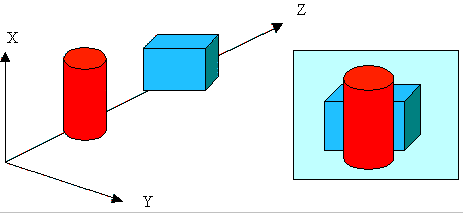
\includegraphics[width=\linewidth]{inc/zbufer.png}
	\end{center}
	\caption{Иллюстрация работы алгоритма Z-буфера}
\end{figure}
\FloatBarrier

К преимуществам алгоритма можно отнести его простоту и отсутствие сортировок.
Но у такого подхода есть и много недостатков: идёт большой перерасход памяти, так как хранятся два двухмерных массива. 
Эффекты прозрачности и просвечивания тяжело реализовать, также возникают проблемы с устранением лестничного эффекта \cite{rojers}.

\subsection{Алгоритм обратной трассировки лучей}
Алгоритм предлагает рассмотреть следующую ситуацию: через каждый пиксел изображения проходит луч, выпущенный из камеры, и программа должна определить точку пересечения этого луча со сценой.
Первичный луч – луч, выпущенный из камеры. 

На рисунке 1.2 представлена ситуация, когда первичный луч пересекает объект в точке H1:
\FloatBarrier
\begin{figure}[h]
	\begin{center}
		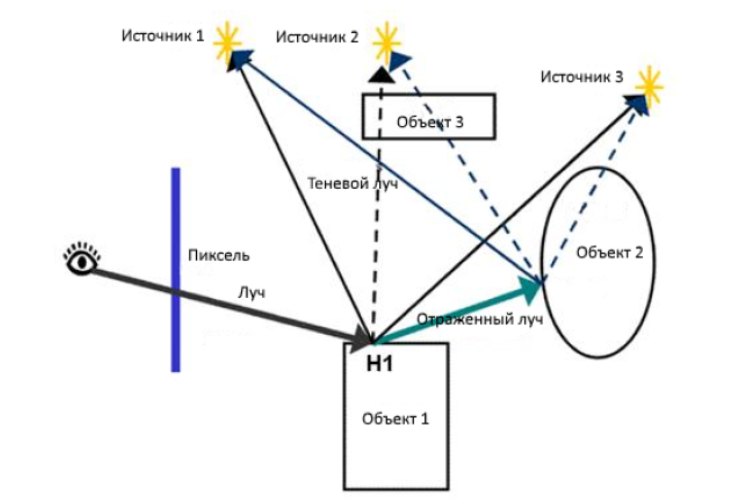
\includegraphics[width=\linewidth]{inc/tras.png}
	\end{center}
	\caption{Иллюстрация работы алгоритма обратной трассировки лучей}
\end{figure}
\FloatBarrier

Для источника света определяется, видна ли для него эта точка. 
Чтобы это сделать, испускается теневой луч из точки сцены к источнику. 
Если луч пересёк какой-либо объект сцены, то значит, что точка находится в тени, и её не надо освещать.
В обратном случае требуется рассчитать степень освещённости точки.

Затем алгоритм рассматривает отражающие свойства объекта: если они есть, то из точки H1 выпускается отражённый луч, и процедура повторяется рекурсивно. 
Тоже самое происходит при рассмотрении свойств преломления.
Этот алгоритм подходит для поставленной задачи, так как полученное изображение соответствует высокому уровню реалистичности.
Также данный метод позволяет учесть все физические явления: отражение, преломление, воссоздание теней. \cite{rojers}

У алгоритма существует недостаток: трассировка лучей каждый раз начинает заново процесс вычисления цвета пиксела, рассматривая каждый луч по отдельности. \cite{raytrac}
При этом временные затраты у алгоритма существенно большие, чем у алгоритма Z-буфера.

\subsection{Вывод}
У программы два режима работы: в первом пользователь добавляет и редактирует объекты, 
изменяет спектральные характеристики, а во втором уже воссоздаётся реалистическое изображение.
В первом режиме важна скорость, поэтому из всех алгоритмов был выбрал Z-буфер. 
Для второго же важна реалистичность, учёт физических и оптических эффектов, и для решения этой задачи был выбран алгоритм обратной трассировки лучей.

\section{Анализ алгоритмов закраски}

\subsection{Метод закраски Гуро}
Метод Гуро устранить дискретность изменения интенсивности и создать иллюзию гладкой криволинейной поверхности. 
Он основан на интерполяции интенсивности \cite{cul}.
Сам алгоритм можно разбить на четыре основных этапа:
\begin{enumerate}
	\item Вычисление нормалей ко всем полигонам.
	\item Определение нормали в вершинах путём усреднения нормалей по всем полигональным граням, которым принадлежит рассматриваемая вершинам.
	На рисунке 1.3 представлен пример вычисления нормали.
	\FloatBarrier
	\begin{figure}[h]
		\begin{center}
			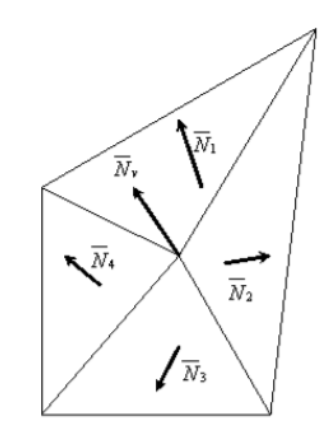
\includegraphics[]{inc/guro.png}
		\end{center}
		\caption{Определение всех нормалей к вершине грани}
	\end{figure}
	\FloatBarrier
	\item Вычисление значения интенсивности в вершинах многоугольника на основе выбранной модели освещения.
	\item Закраска каждого многоугольника путём линейной интерполяции в вершинах сначала вдоль рёбер, а затем и между ними.
\end{enumerate}

Метод Гуро применим для небольших граней, расположенных на значительном расстоянии от источника света. 
Если же размер грани большой, то расстояние от источника света до центра будет меньше, чем до вершин, и центр грани должен выглядеть ярче, чем рёбра.
Но из-за линейного закона, используемого в интерполяции, метод не позволяет это сделать, поэтому появляются участки с неестественной освещённостью \cite{rojers}.

\subsection{Вывод}
Вместе с алгоритмом z-буфера будет использоваться метод Гуро, так как он быстрый, и получается приемлемое качество изображения, в том числе можно заметить сглаживание тел. 
При создании реалистичного изображения будет использоваться алгоритм обратной трассировки лучей, который не требует какого-то ещё дополнительного алгоритма закраски.

\section{Анализ алгоритмов моделирования освещения}
Реалистичность изображения во многом зависит от правильного выбора алгоритма освещения. 
Все модели освещённости можно разделить на две группы: глобальные и локальные. 
Локальные модели учитывают только первичный источник света, а глобальные также рассматривают физические явления: 
отражение света от поверхностей, преломление света.

\subsection{Модель Ламберта}
В этой модели воспроизводится идеальное диффузное освещение. \cite{cul}
Свет при попадании на поверхность равномерно рассеивается во все стороны. 
При расчёте учитывается только ориентация нормали поверхности (нормаль $\overline{N}$ ) и направление на источник света (вектор $\overline{L}$).
Пусть $I_d$ – рассеянная составляющая освещённости в точке, $K_d$ – свойство материала воспринимать рассеянное освещение, 
$I_0$ – интенсивность рассеянного освещения. 

Тогда интенсивность можно рассчитать по формуле:
\begin{equation}
I_d = K_d(\overline{L}, \overline{N})I_0
\end{equation}

Модель Ламберта является одной из самых простых моделей освещения. Она часто используется в комбинации с другими моделями, так как практически в любой можно выделить диффузную составляющую. Равномерная часть освещения чаще всего представляется именно моделью Ламберта \cite{light}.

\subsection{Модель Фонга}
Модель Фонга основывается на предположении, что освещённость каждой точки можно разбить на три компоненты \cite{light}:
\begin{itemize}
	\item Фоновое освещение (ambient) – оно присутствует на любом участке сцены, не зависит от источников света, потому считается константой;
	\item Рассеянный свет (diffuse) – рассчитывается также, как в модели Ламберта;
	\item Бликовая составляющая (specular) – зависит от того, насколько близко находятся вектор отражённого луча и вектор до наблюдателя.
\end{itemize}

Свойства источника определяют мощность излучения для каждой из компонент, а свойства материала – способность объекта воспринимать свет.


Пусть $ \overline{N} $ – вектор нормали к поверхности в точке, $ \overline{L} $ – падающий луч, $ \overline{R} $ – отражённый луч,
$ \overline{V} $ – вектор, направленный к наблюдателю, $ k_a $ – коэффициент фонового освещения, $ k_d $ – коэффициент диффузного освещения, 
$ k_s $ – коэффициент зеркального освещения, p – степень, аппроксимирующая пространственное распределение зеркально отражённого света.
Тогда интенсивность света подсчитывается формулой 1.2:

\begin{equation}
	I_a = K_a * I_a + K_d(\overline{N}, \overline{L}) +  K_s(\overline{R}, \overline{V})^p
\end{equation}

На рисунке 1.4 приведён пример работы модели Фонга:
\FloatBarrier
\begin{figure}[h]
	\begin{center}
		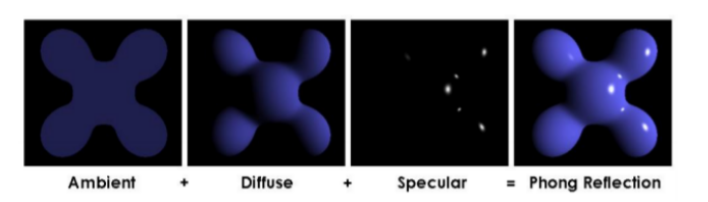
\includegraphics[width=\linewidth]{inc/fong.png}
	\end{center}
	\caption{Иллюстрация работы модели Фонга}
\end{figure}
\FloatBarrier

\subsection{Модель Уиттеда}
Эта модель освещения позволяет рассчитать интенсивность отражённого к наблюдателю луча в каждом пикселе изображения. 
Используемый в проекте вариант учитывает также свет от других объектов сцены или пропущенный сквозь них. \cite{light}
Помимо направления взгляда, отражённого луча, источника света, также рассматривается и составляющая преломления. \cite{raytrac}

Пусть $ K_a $ – коэффициент рассеянного отражения,$ K_d $ – коэффициент диффузного отражения, $ K_s $ – коэффициент зеркальности, $ K_r $ – коэффициент отражения, 
$ K_t $ – коэффициент преломления, $ I_a $ – интенсивность фонового освещения, $ I_d $ – интенсивность для диффузного рассеивания, 
$ I_s $ – интенсивность для зеркальности, $I_r$ - интенсивность излучения, приходящего по отраженному лучу, $ I_t$ интенсивность излучения, приходящего по преломленному лучу, $С$ - цвет поверхности.

Тогда интенсивность по модели Уиттеда можно рассчитать по формуле 1.3:
\begin{equation}
I = K_aI_aC + K_dI_dC + K_sI_s + K_rI_r + K_tI_tС
\end{equation}

\subsection{Вывод}
Для первого режима работы лучше подходит модель Ламберта, так как она быстрее и эффективно сочетается с Z-буфером. 
Для создания реалистического изображения выбрана модель Уиттеда, потому что здесь в первую очередь важно качество полученного изображения, 
и этот способ показывает высокую эффективность в комбинации с обратной трассировкой лучей.

\section{Перспективно-корректное текстурирование объектов трёхмерной сцены}
Пусть  $u$, $v$ -- координаты текстуры, которые требуется найти для решения задачи наложения текстур на объект трёхмерной сцены.
Метод перспективно-корректного текстурирования основан на приближении $u$ и $v$ кусочно-линейными функциями.
При отрисовке каждая сканирующая строка разбивается на части, в начале и конце каждого куска вычисляются точные значения
$u$ и $v$, а внутри каждой части применяется линейная интерполяция. \cite{rojers}

Пусть $s_x$ и $s_y$ -- координаты, принадлежащие проекции текстурируемого треугольника.
Тогда значения $ \frac{1}{z} $, $ \frac{u}{z} $ и $ \frac{v}{z} $ линейно зависят от $s_x$ и $s_y$.
Следовательно, для каждой вершины достаточно подсчитать значения $ \frac{1}{z} $, $ \frac{u}{z} $ и $ \frac{v}{z} $ и
линейно их интерполировать.

Точные значения $ u $ и $ v $ подсчитываются по формуле 1.4ы: 
\begin{equation}
u = \frac{(u/z)}{1/z},  v = \frac{(u/z)}{1/z} 
\end{equation}

\section{Алгоритм заполнения треугольника с использованием барицентрических координат}
Барицентрические координаты -- это координаты, в которых точка треугольника описывается как линейная комбинация вершин. \cite{rojers}

В работе используется нормализованный вариант: суммарный вес трёх вершин равен единице:
\begin{equation}
\begin{aligned}
& p = b_ov_0 + b_1v_1 + b_2v_2 \\ 
&b_0 + b_1 + b_2 = 1
\end{aligned}
\end{equation} 
Такой выбор обусловлен тем, что барицентрические координаты легко вычислить, так как они равны отношению площадей треугольников, которые образует точка внутри треугольника и вершина, к общей площади треугольника.

Третья координата вычисляется через свойство нормировки, то есть фактически имеется только две степени свободы.

Барицентрические координаты позволяют интерполировать значение любого атрибута в произвольной точке треугольника: значение атрибута в заданной точке треугольника равно линейной комбинации барицентрических координат и значений атрибута в соответствующих вершинах:
\begin{equation}
	T = T_0b_0 + T_1b_1 + T_2b_2
\end{equation}

Алгоритм закраски с использованием барицентрических координат состоит из двух этапов:
\begin{enumerate}
	\item Поиск прямоугольника, минимального по площади, чтобы он содержал в себе рассматриваемый треугольник.
	\item Сканирование прямоугольника слева направо и вычисление барицентрических координат для каждого выбранного пикселя. Если значение координат находится в промежутке от 0 до 1, и сумма по всем координатам не превышает 1, то пиксель закрашивается.
\end{enumerate}

\section{Вывод}
Было приведено описание модели трёхмерного объекта в сцене,
рассмотрены формализация объектов сцены и требования к работе программы.
Рассмотрены алгоритмы построения трёхмерного изображения, методы закраски, модели освещения, а также способы тексуризации и закраски треугольников.